\documentclass[11]{article}
\usepackage{graphicx}
\graphicspath{ {images/} }


\title{CS2006 Haskell Project 2 - \\ Gomoku}
\date{27/04/2018}
\author{Matriculation Numbers: 160001362, 160016245, 160021429 (Group 14)}

\begin{document}
	\maketitle
	\newpage
	\tableofcontents
	
	\newpage
	\section{Summary of Functionality}
		This practical specified the development of the board game Gomoku using the functional programming language Haskell. \\\\The provided README file gives detailed instructions explaining how to execute the program including configuring settings both through the terminal as well as in game.
\\\\The following functionality has been implemented:
	\subsection{Basic Specification:}
		All requirements from the basic specification have been implemented. They are as follows:	
		\begin{enumerate}
			\item \textbf{Implement the game mechanics in Board.hs} - For this requirement code in this file enables the board and world initialisation, and works out who has won by counting pieces to check for a win condition.
			\item \textbf{Implement the drawWorld function in Draw.hs to display the current board state graphically} - The Draw.hs file uses Picture objects (included from the gloss graphics dependency) to display the assets required for the game (currently using a combination of bitmap images stored in the world and rendered images) which are refreshed ten times a second from playIO in the Main.hs file.
			\item \textbf{Implement appropriate event handlers for inputs events} - The Input.hs file runs a handleInput function when the user clicks part of the display which decides which action to take depending on whether the area clicked is a button or part of the game board. Depending on the current game state, a different action will be take. For example if the game mode is player vs player, a different piece will be played depending on the current turn.
			\item \textbf{Implement a move generator (in AI.hs) and an evaluation function (in Board.hs) to provide a computer opponent} - two AIs have been implemented, a random AI and a heuristic based AI. The random AI generates a random index to refer to an element in a list of empty positions of the board and places a piece there. The heuristic AI uses the evaluation function in Board.hs to calculate its board score relative to its opponent for each possible move and chooses the highest scoring move. The board score for the heuristic AI is determined by the number of continuous sets the AI has, the average length of these sets, the max length set on the current board, and the number of sets which have been blocked by the other player.
		\end{enumerate}
	
	\subsection{Additional Requirements:}
	 From the suggested additional requirements, all of the easy and medium requirements have been implemented, as have the listed hard requirements:
	 	\subsubsection{Easy}
			\begin{itemize}
				\item \textbf{Easy Requirement 1} - The ability to enter command line arguments to set up the game options has been implemented by altering the initWorld function to take parameters relating to each setting. The parameters that can be set are:
					\begin{itemize}
						\item Board size.
						\item Target (i.e. number in a row to win).
						\item Player colour (White/Black).
						\item Game type (normal or rule of four and four).
						\item AI mode (beginner - random, intermediate - heuristic AI, pvp - player vs player).
					\end{itemize}
				\item \textbf{Easy Requirement 2} - When the undo button is clicked in-game, an undo event is triggered which calls a funtion in Board.hs to roll back the game by two moves (to the previous player move).
				\item \textbf{Easy Requirement 3} - The rule variant four and four has been implemented in Board.hs. When the player tries to place a piece it simulates the board move and checks whether the checkFourAndFour function returns True. It calls functions which check each piece on the simulated board individually for the number of combinations of four in a row. Since every piece is checked individually, a row of four pieces would return the number four. If the total number is higher than four, it means that there are more than two open rows of four in a row if the move is made. It returns true and thus blocks all of these moves from happening. 
			\end{itemize}

		\subsubsection{Medium}
			\begin{itemize}
				\item \textbf{Medium Requirement 1} - In addition to the ability to set options via the command line as described previously, game options can also be set in-game using a series of buttons. These buttons are declared in Board.hs and are stored in the the World state. As suggested by the specification, when the settings are not set in the command line, handleInput detects that the settings/loading screen should be displayed to allow the user to configure the game options. 
				\item \textbf{Medium Requirement 2} - Bitmap images are loaded in during the execution of Main.hs from the Assets/ folder located within the Code/ directory. They are then stored in the the World state as lists of Picture objects and are then utilised from within the Draw.hs file when different aspects of the game are displayed.
				\item \textbf{Medium Requirement 3} - A hint button has been implemented which can be toggled on or off by the user during the game. When toggled on a pink/red piece is displayed on a position on the board determined by the evaluate function in Board.hs (the same one used by the AI) which is deemed to be a favourable move for the player.
				\item \textbf{Medium Requirement 4} - Save and load buttons have been created in Board.hs and stored in the World state which respectively trigger save and load events which result in the current board size, board target, game type, and board pieces to be written to, or read from, the save.dat file contained in the Code/ directory.
			\end{itemize}
		\subsubsection{Hard}
				\begin{itemize}
					\item \textbf{Hard Requirement 2} - As discussed previously, our implementation has two distinct AI opponents, one which selects moves based on a pseudo random index, and one which selects moves based on a heuristic which generates a score for each possible board state when a move is made. One of our game options as described in both the first easy and first medium requirements is the AI mode which allows the user to choose between each of these opponents.
				\end{itemize}
	\subsection{Further Features:}
		The following additional features have also been implemented:
		\begin{itemize}
			\item \textbf{Player vs Player } - In addition to the basic and additional requirements, the ability to play a game against a human opponent has also been implemented and is selected in the same way as each of the AI opponents. When setting the command line option for the AI mode the keyword "pvp" can be used, or alternatively this can be selected using the pvp button in the user interface.
		\end{itemize}
		
	\section{Evidence of Testing}	
		The testing of the game was carried out iteratively as features were developed to ensure that they worked and complied with the rest of the system. Examples of testing of the main features of the program (that are visually demonstrable) have had screen-shots taken which are included in the \textbf{appendix} section at the end of the report. The screen-shots show the settings menu, the command line being used to set the game options, an example game between the player and the random AI, an example game between the player and the heuristic AI, an example player versus player game, an example of the game state being saved, and finally an example of the four and four condition being met.
	\section{Known Problems}
		\begin{itemize}
			\item \textbf{Solving Gomoku} - At the moment the heuristic based AI is able to beat the user all of the time on a game of three in a row if they go first (as far as testing has shown). However for games with a target higher than three in a row the AI performs well but could be improved to the point where the player can no longer win. The Dutch Computer Scientist Victor Allis has shown in his dissertation\footnote{http://fragrieu.free.fr/SearchingForSolutions.pdf} AI solutions for various games including Connect Four, Qubic, and relevant to this practical, Gomoku. To improve the AI a search tree could be implemented which uses the techniques discussed in this literature.
			\item \textbf{Improving Hints} - Further to the previous point, as the hint feature uses the evaluate function used by the AI, the hints are only as good as the AI. The hints would also therefore improve as improvements to the AI are made.
		\end{itemize}
		
	\section{Problems Overcome}
		\begin{itemize}
			\item \textbf{CPU Performance} - Initially our solution resulted in an incredibly high CPU utilisation which turned out to be as a result of an infinite loop being triggered each time a button (or area of the display) was clicked. The loop seemed to be triggered in order to handle incoming input from the user. In order to avoid these infinite loops we changed the way in which the handleInput function returned values.
			\item \textbf{Memory Usage} - For a large part of the development of the program, performance would greatly diminish with time as the program continued to run. Initially we though this to be an issue with the way the pieces were counted or with how the AI evaluated the board. Unbeknownst to us, it was actually a result of the way the program displayed the bitmap images. Rather than loading them in once at the start of the program and reusing them (as is the case now) the program would load in all of the images every time the display refreshed, resulting in memory to be filled up storing additional copies of the images. Eventually this would result in a system crash when there was no additional memory for the images. The solution to this was to add fields in the World state to store the images and then access them from there.
		\end{itemize}

	\section{Summary of Provenance}
			The source files modified for this practical are the original five provided (AI.hs, Board.hs, Draw.hs, Input.hs, Main.hs) and now include the code required for each of the following requirements:
			\begin{itemize}
				\item 160001362:
					\begin{itemize}
						\item \textbf{Basic Requirement 4 (AI.hs, Board.hs)}
						\item \textbf{Medium Requirement 3 (Board.hs)} - Implemented the evaluation for the AI which is also used to generate a user hint.
						\item \textbf{Hard Requirement 2 (AI.hs)} - Implemented the multiple AIs
					\end{itemize}
					
				\item 160016245:
					\begin{itemize}
						\item \textbf{Easy Requirement 1 (Main.hs)}
						\item \textbf{Easy Requirement 3 (Board.hs)} - Rule of four and four
						\item \textbf{Medium Requirement 1 (Main.hs, Board.hs, Draw.hs, Input.hs)}
						\item \textbf{Medium Requirement 3 (Draw.hs)} - Displayed the hints generated by the evaluation function.
						\item \textbf{Hard Requirement 2 (Main.hs, Board.hs, Input.hs)} - Enabled user to choose between the AI modes (as well as player vs player).
					\end{itemize}
					
				\item 160021429:
					\begin{itemize}
						\item \textbf{Basic Requirements 1 - 3 (Board.hs, Draw.hs, Input.hs, Main.hs)}
						\item \textbf{Easy Requirement 2 (Board.hs, Input.hs, Draw.hs)}
						\item \textbf{Medium Requirement 2 (Board.hs, Draw.hs)}
						\item \textbf{Medium Requirement 4 (Board.hs, Input.hs, Draw.hs)}
					\end{itemize}
			\end{itemize}
				
	
\section{Conclusion}
	Overall we have successfully implemented the board game Gomoku in the functional programming language Haskell. Our solution satisfies all basic, easy, and medium requirements, as well as the second hard requirement and the additional feature of the player vs player game mode.\\\\Given more time we would implement the rest of the medium/hard and hard requirements and improve upon our current solution by altering the way in which the AI moves and hints are generated, perhaps using some combination of minimax and alpha beta pruning, or maybe even by replicating the solutions laid out in Victor Allis' dissertation.


  	\begin{thebibliography}{1}
  		\bibitem{lit1} Victor Allis, 
  		\textit{"Searching for Solutions in Games and Artificial Intelligence"}, 
  		Maastricht University, 
  		http://fragrieu.free.fr/SearchingForSolutions.pdf, 
  		(1994).
  	\end{thebibliography}
  	\newpage
\section{Appendix}
	\begin{figure}[h]
					\caption{Options/Settings Screen if no command line arguments are given:}				\centering
					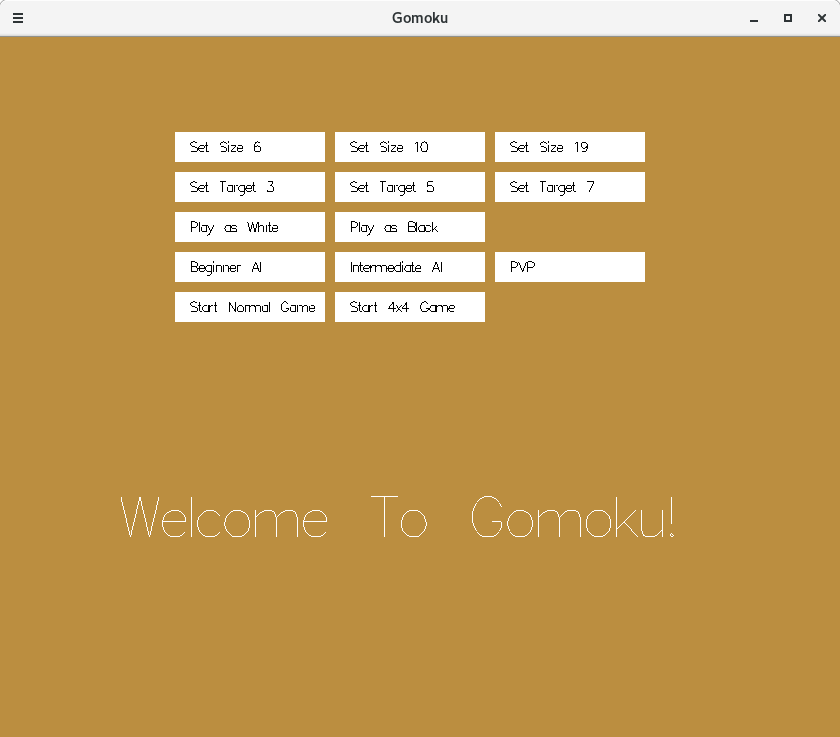
\includegraphics[scale=0.5]{SettingsScreen.png}
		\end{figure}

\begin{flushleft}
	Example of options being set via the command line:

\includegraphics[scale=0.6]{CommandLineArguments.png}
\end{flushleft}

\newpage

\begin{figure}[h]
					\caption{Player vs Random: AI is black and plays first:}				\centering
					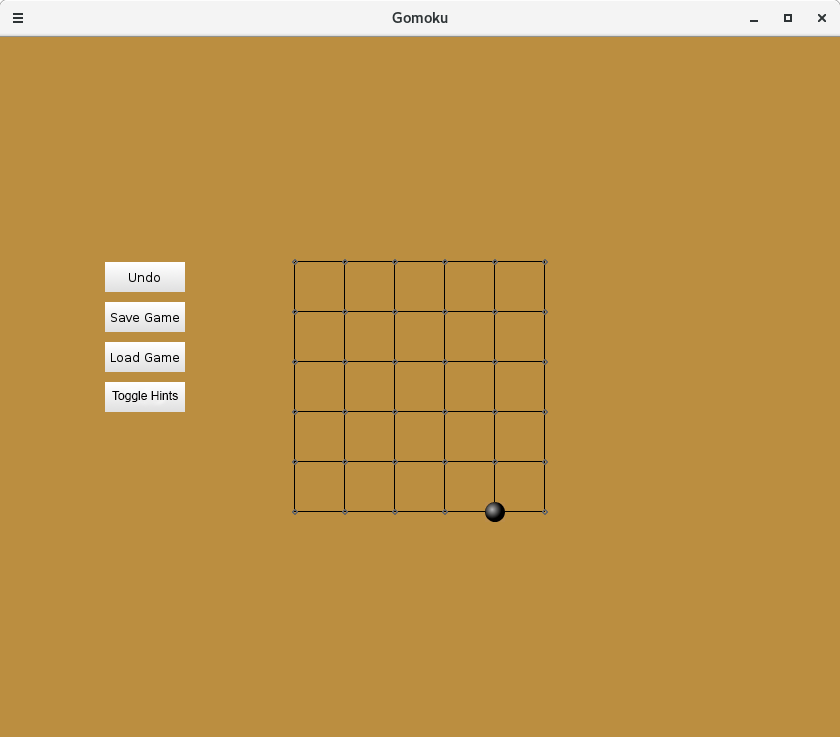
\includegraphics[scale=0.5]{Random1.png}
\end{figure}

\begin{figure}[h]
					\caption{Player vs Random:}				\centering
					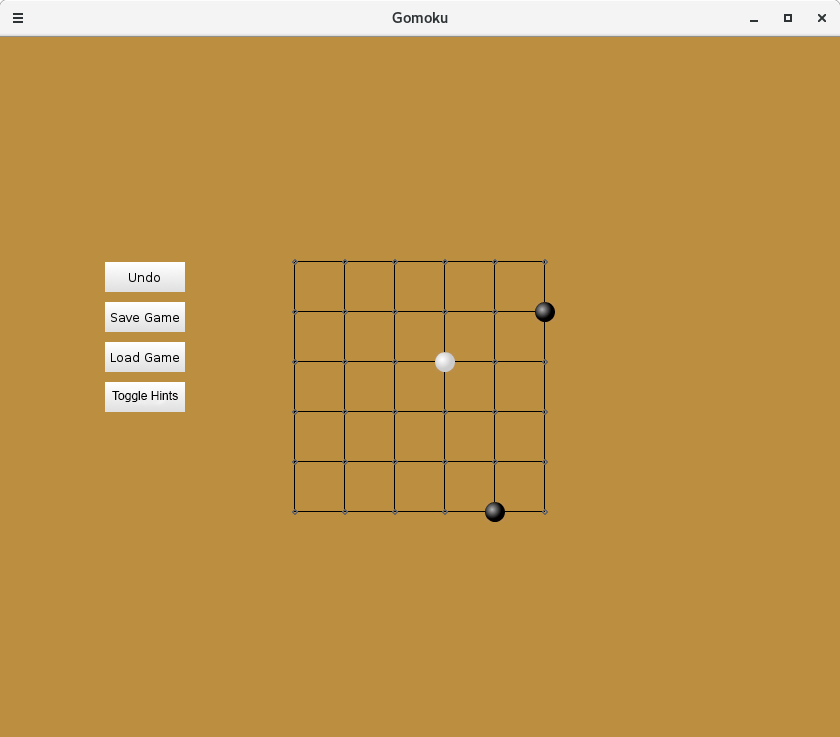
\includegraphics[scale=0.5]{Random2.png}
\end{figure}

\begin{figure}[h]
					\caption{Player vs Random:}				\centering
					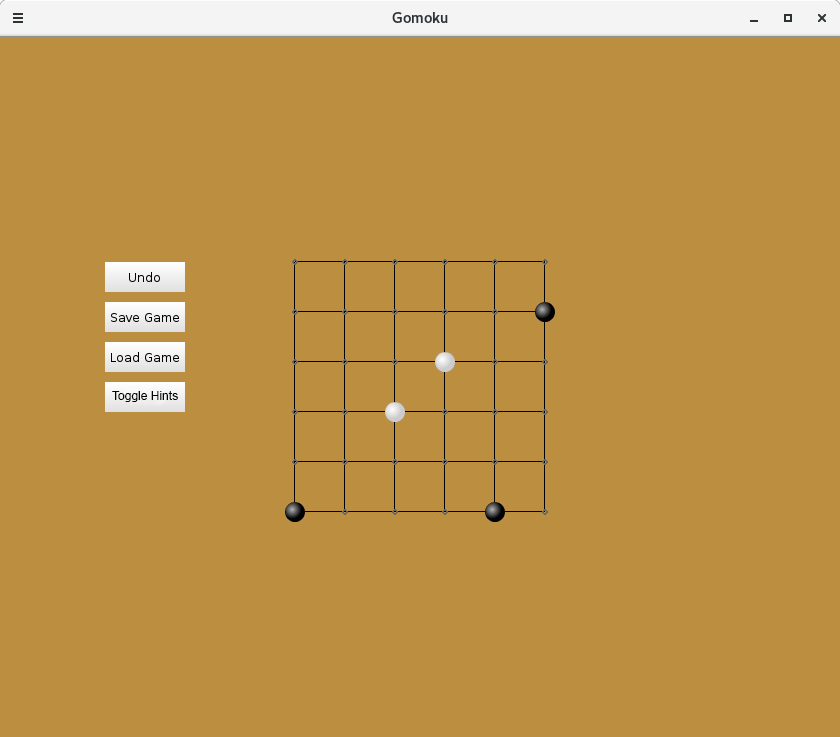
\includegraphics[scale=0.5]{Random3.png}
\end{figure}

\begin{figure}[h]
					\caption{Player vs Random - white (player) gets three in a row and wins:}				\centering
					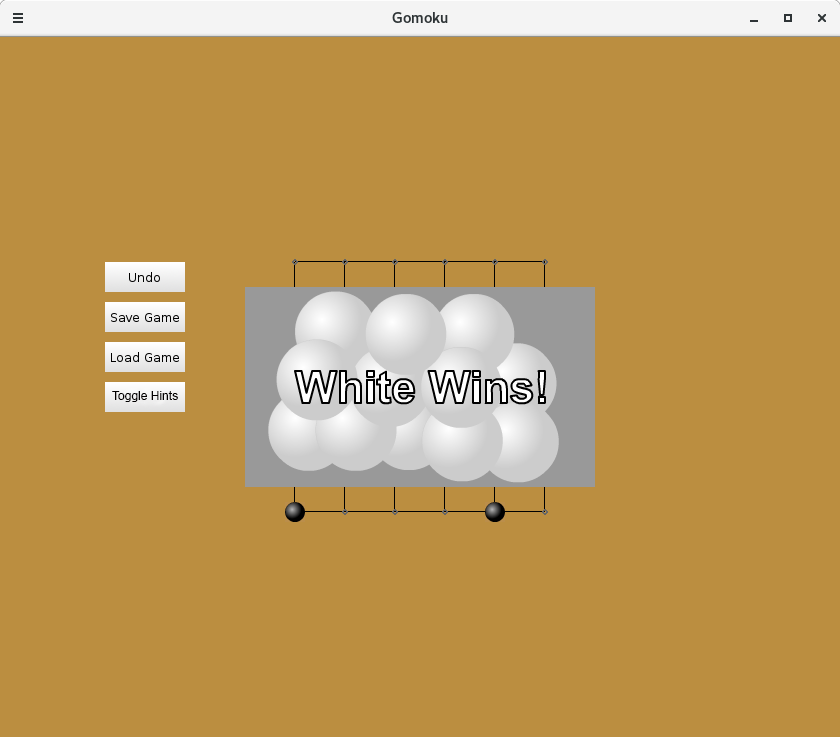
\includegraphics[scale=0.5]{Random4.png}
\end{figure}

\begin{figure}[h]
					\caption{Player vs Heuristic: AI is black and plays first:}				\centering
					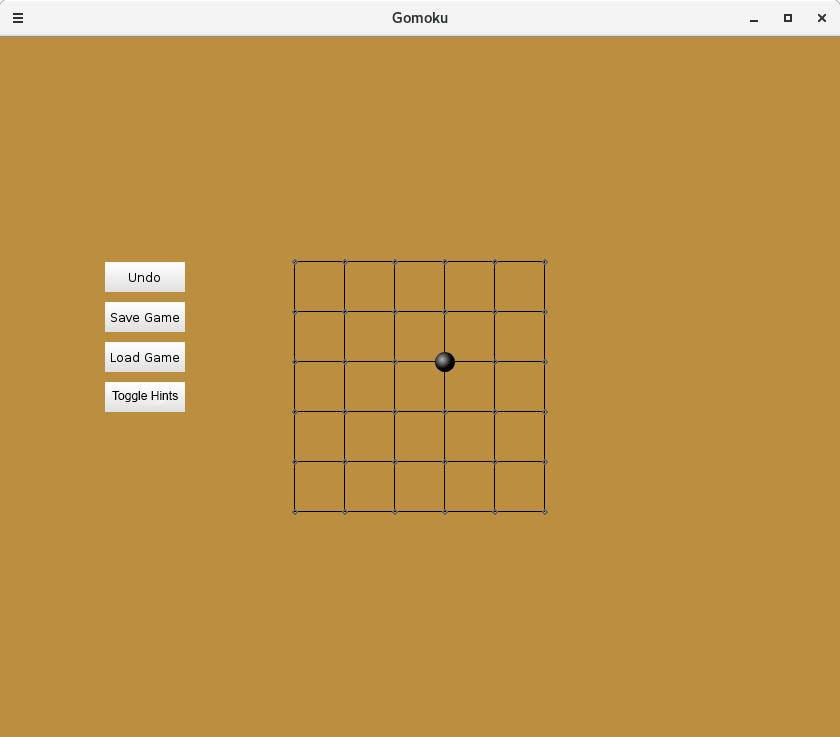
\includegraphics[scale=0.5]{Heuristic1.png}
\end{figure}

\begin{figure}[h]
					\caption{Player vs Heuristic (hints toggled on by player, displayed as red/pink piece):}				\centering
					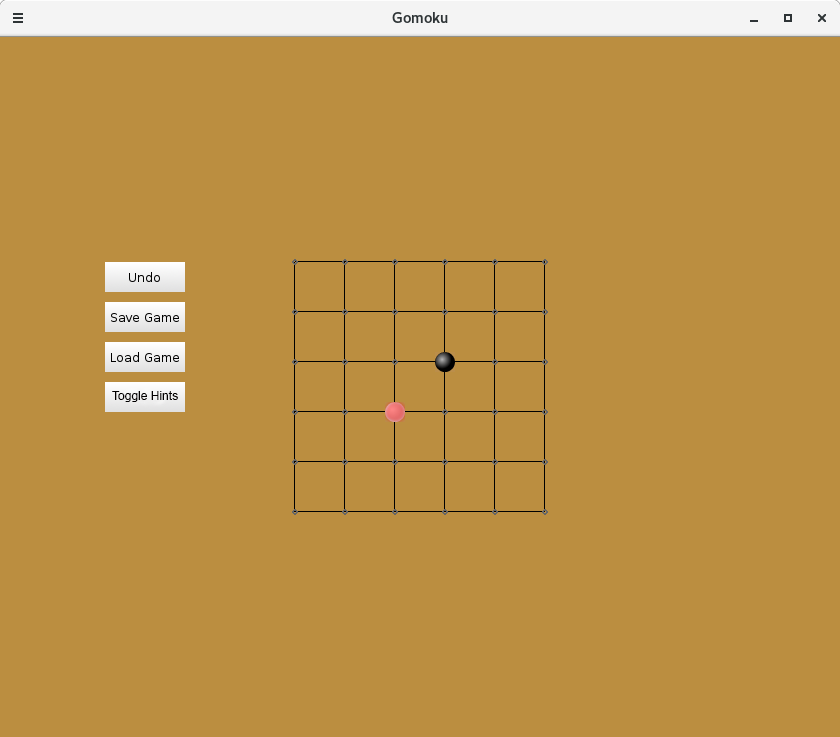
\includegraphics[scale=0.5]{Heuristic2.png}
\end{figure}

\begin{figure}[h]
					\caption{Player vs Heuristic:}				\centering
					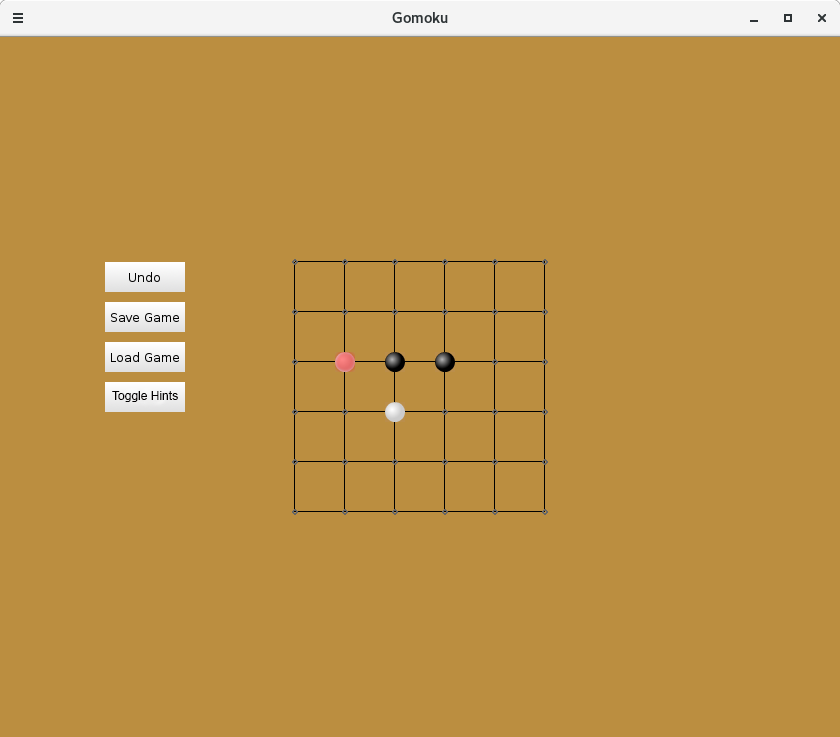
\includegraphics[scale=0.5]{Heuristic3.png}
\end{figure}

\begin{figure}[h]
					\caption{Player vs Heuristic - white (player) gets three in a row and wins (black AI on three in a row always beats player):}				\centering
					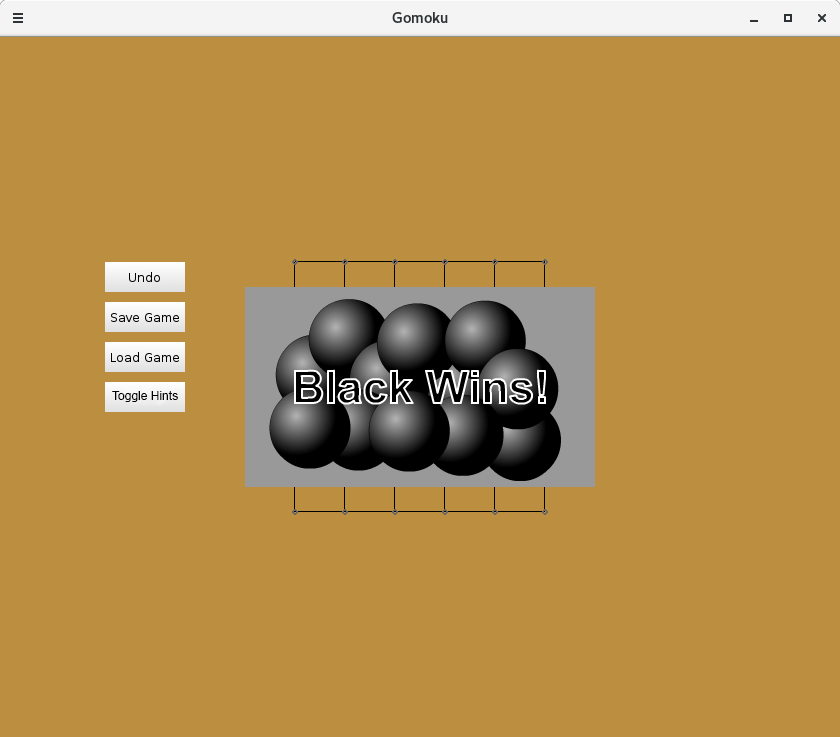
\includegraphics[scale=0.5]{Heuristic4.png}
\end{figure}

\begin{figure}[h]
					\caption{Player vs Player (example of 10x10 board):}				\centering
					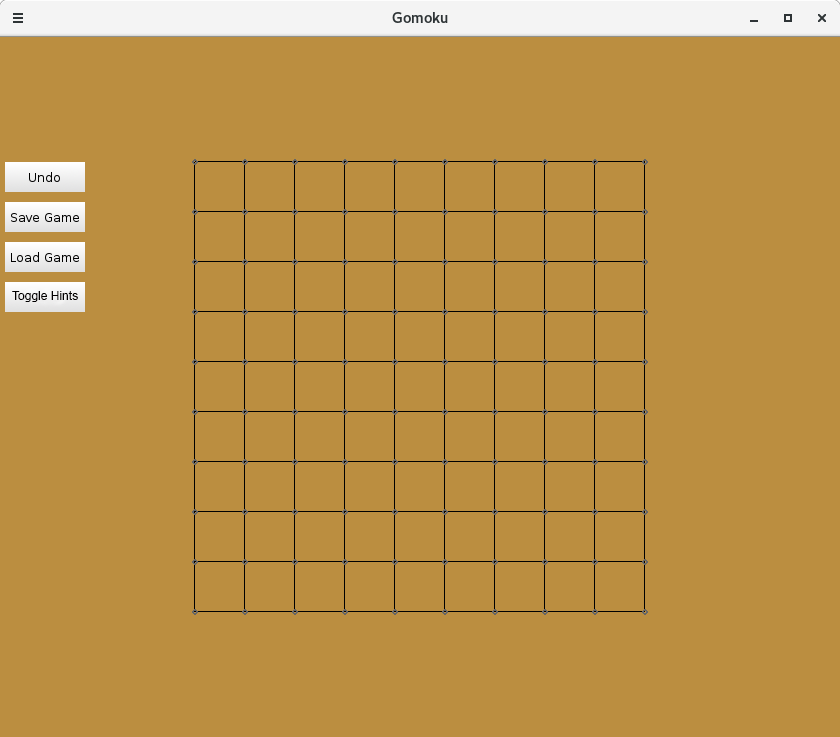
\includegraphics[scale=0.5]{pvp1.png}
\end{figure}

\begin{figure}[h]
					\caption{Player vs Player (black just about to win):}				\centering
					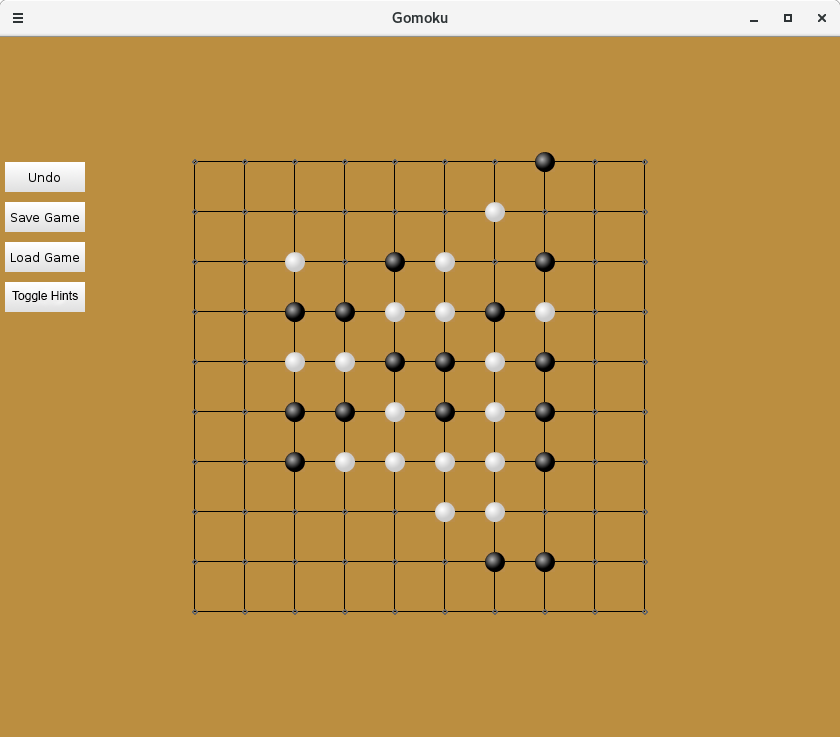
\includegraphics[scale=0.5]{pvp2.png}
\end{figure}

\begin{figure}[h]
					\caption{Player vs Player (Black wins by getting five in a row):}				\centering
					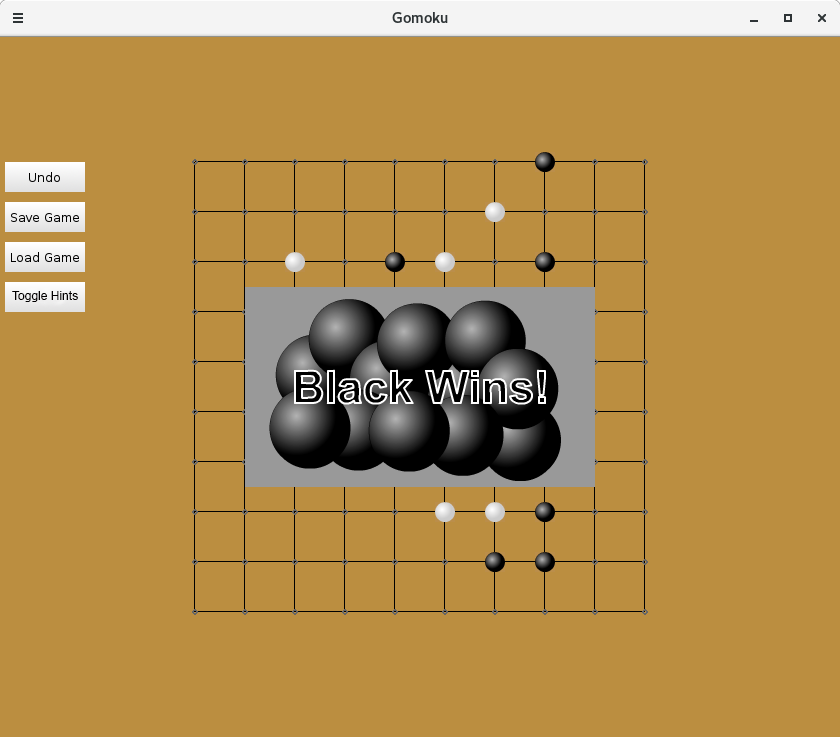
\includegraphics[scale=0.5]{pvp3.png}
\end{figure}

\begin{figure}[h]
					\caption{Example of Save Game- Game state to be saved:}				\centering
					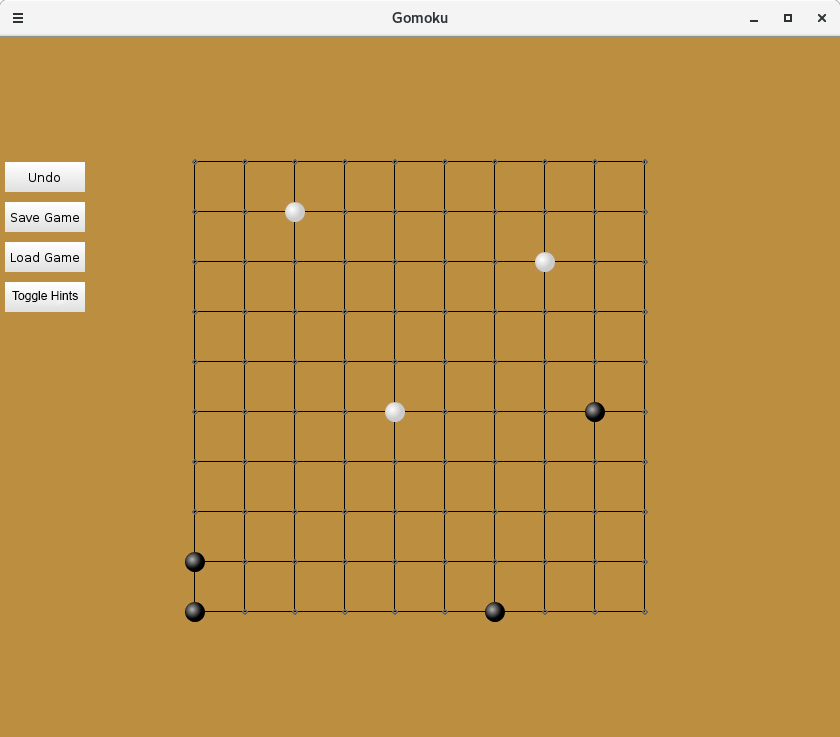
\includegraphics[scale=0.5]{save1.png}
\end{figure}

\begin{figure}[h]
					\caption{Example of Save Game- Save game file:}				\centering
					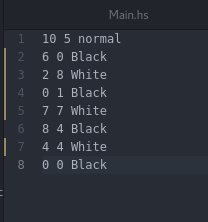
\includegraphics[scale=0.5]{save2.png}
\end{figure}

\begin{figure}[h]
					\caption{Four and Four Condition (black can't get a horizontal four in a row):}				\centering
					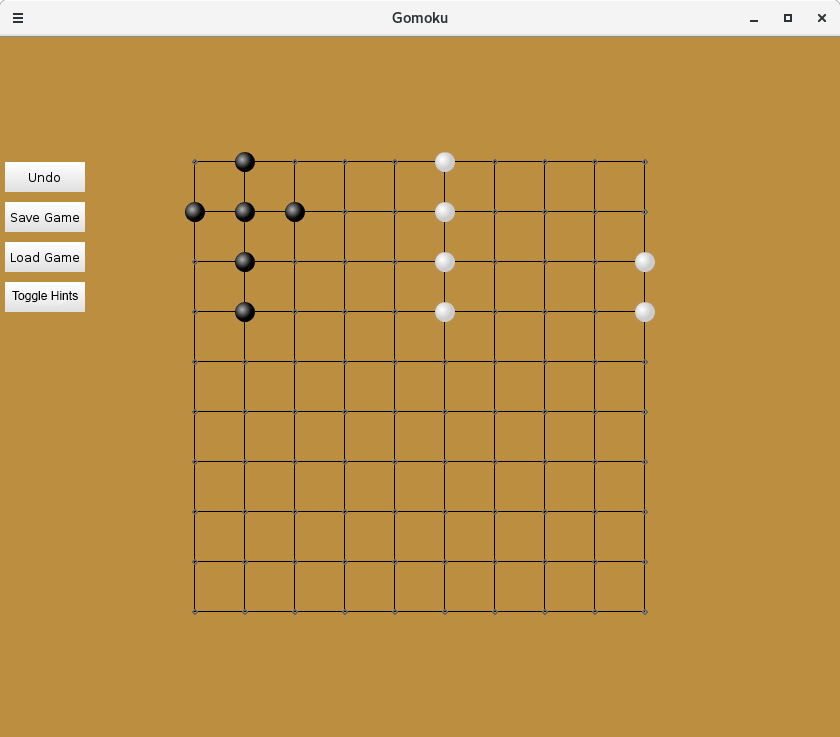
\includegraphics[scale=0.5]{FourAndFour.png}
\end{figure}

\newpage

		


		
	

\end{document}